\documentclass[oneside,AutoFakeBold]{nccuthesis} %如果要撰寫中文論文,請在[oneside]後面加上[zh]即可

\usepackage{times}
\usepackage{verbatim}
\usepackage{color}
\usepackage{url}
\usepackage{graphicx}
\usepackage{array}
\usepackage{pdfpages} % include outside .pdf
\usepackage{wallpaper} % watermark
\usepackage{etoolbox}
\usepackage{enumitem}


% for table generate
\usepackage{mathtools}
\usepackage{amsmath}
\usepackage{amssymb}
\usepackage{booktabs}
\usepackage{adjustbox}
\usepackage{multicol}
\usepackage{multirow}

% Format the refs
\usepackage[style=apa,sortcites=true,sorting=nyt,backend=biber]{biblatex} % 想換成其他引用格式的話,請參考https://www.overleaf.com/learn/latex/Biblatex_citation_styles的指示,把style=apa換成你需要的格式。例:如果要用MLA就換成style=mla。
\addbibresource{bibliography.bib}
\usepackage[hidelinks]{hyperref}

%文內的各種連結都可以設定顏色
%這個只是示範用,學校的規定應該都是要用黑色的
%\hypersetup{
    %colorlinks = true, % 設定連結的顏色
    %linkcolor= black, % 文內連結
    %citecolor = magenta, % citation連結的顏色
    %urlcolor=blue % 超連結的顏色
%}

% For the tree
\usepackage{tikz}
\usepackage{tikz-qtree}

% For barchart
\usepackage{pgfplots}

% Using the tex-text mapping for ligatures etc.
\defaultfontfeatures{Mapping=tex-text}

% Set the default fonts
\setmainfont{Times New Roman}
\setCJKmainfont{TW-Kai}

% For glossing
\usepackage{gb4e}
\usepackage{langsci-gb4e}
\newcommand{\pream}[1]{#1:\\[-4.5ex]} % for preamble lines, supplies a colon and removes some vertical space
\newcommand{\pglt}{\vspace*{-2ex}\glt} % for use in examples that have a preamble


% Your information goes here
% author: Tz-Huan Huang [http://www.csie.ntu.edu.tw/~tzhuan]

% ----------------------------------------------------------------------------
% "THE CHOCOLATE-WARE LICENSE":
% Tz-Huan Huang wrote this file. As long as you retain this notice you
% can do whatever you want with this stuff. If we meet some day, and you think
% this stuff is worth it, you can buy me a chocolate in return Tz-Huan Huang
% ----------------------------------------------------------------------------

% Syntax: \var{English}{Chinese} 前面打英文,後面打中文
\university{National Chengchi University}{國立政治大學}
\college{College of Foreign Languages \& Literature}{外國語文學院}
\institute{Graduate Institute of Linguistics}{語言學研究所}
\type{Master's Thesis / Doctoral Dissertation}{碩士論文/博士論文} % 你的學位
\title{This is the Title of the Thesis}{論文標題} % 你的題目
\author{Noam}{諾姆} % 你的名字
\advisor{Chomsky}{喬姆斯基 博士} % 指導教授
\defenseyear{2022}{111} % 中文年份
\defensemonth{June}{6} % 英文年份
\defenseday{15} % 日期

\pgfplotsset{compat=1.14}
\begin{document}

% 政大論文浮水印
\input{with-watermark.tex} % 如果不需要浮水印可以將此行刪除

\hypersetup{pageanchor=false}

\frontmatter
\makecover

\clearpages


% generate certification
% \makecertification
% or include scanned pdf
\addcontentsline{toc}{chapter}{口試委員會審定書}
\includepdf[pages={1}]{pdfs/cert.pdf} % 請把pdfs這個資料夾中的cert檔按刪掉,將自己口試委員會審定書的pdf檔命名為cert上傳到該資料夾中即可完成這個頁面的設定。
\clearpage


\setcounter{page}{1}
\hypersetup{pageanchor=true}
\pagenumbering{roman}
\phantomsection


\thispagestyle{plain}
\pagenumbering{roman}
\setcounter{page}{3}
\begin{center}

\vspace*{\fill}
\linespread{1.2}
\Large{\textbf{Copyright \textcopyright \ 2022}}\\
\Large{\textbf{(Your Name)}}\\
\Large{\textbf{All Rights Reserved}}\\

\end{center}

\clearpage
\clearpage

% 看你想寫英文還是中文,可以選擇一個,把另外一個刪掉,因為只能有一頁喔~~

\begin{acknowledgementszh}
這是你用來感謝大家的頁面,想要開始謝謝大家的話請找到acknowledgements.tex這個檔案。反正謝謝大家一定不是一開始就會寫,所以請移步到摘要的頁面看更詳細的介紹~\par
感謝...

感謝\ldots
\end{acknowledgementszh}

\begin{acknowledgementsen}
This is your English acknowledgement. This is your English acknowledgement. This is your English acknowledgement. This is your English acknowledgement. This is your English acknowledgement. This is your English acknowledgement. This is your English acknowledgement. This is your English acknowledgement. This is your English acknowledgement. This is your English acknowledgement. This is your English acknowledgement.

I'm glad to thank\ldots 
\end{acknowledgementsen}


% Table of Content
\clearpages
\tableofcontents % 生成目錄,如果希望可以呈現到標題第二層就好的話,就到nccuthesis.cls的第126行把2改成3
\addcontentsline{toc}{chapter}{Table of Contents}
% List of Figures
\clearpages
\listoffigures
\addcontentsline{toc}{chapter}{List of Figures}
% List of Tables
\clearpages
\listoftables
\addcontentsline{toc}{chapter}{List of Tables}



% Abstract


\begin{abstractzh}
歡迎使用該模板,請在檔案目錄中找到abstract.tex這個檔案以開始編輯你的摘要。在\LaTeX 當中,文字的編輯通常都是在tex檔中完成。為了編輯方便,本模板將論文中的各個章節獨立成檔再透過thesis.tex將它們整合。在開始之前請先確認自己的論文需要以中文撰寫還是英文撰寫。如果要以中文撰寫的話,請找到thesis.tex並根據第一行 \  \% 符號後的指示修改檔案。如果要以英文撰寫的話可以跳過這個步驟。正文的每個章節都被放在chapters/這個資料夾裡面,所以為了開始撰寫本文,請移步到introduction.tex。而封面頁和標題頁的部分請到title.tex當中修改;版權頁請選擇copyright.tex;口試委員會審定書請至thesis.tex的第77行查看;目錄你什麼都不用做就會自己跑出來了。\\

\vspace{\fill}

\noindent
關鍵字:關鍵字1號,關鍵字2號
\end{abstractzh}



\begin{abstracten}
This is your abstract. This is your abstract. This is your abstract. This is your abstract. This is your abstract. This is your abstract. This is your abstract. This is your abstract. This is your abstract. This is your abstract. This is your abstract. This is your abstract. This is your abstract. This is your abstract. This is your abstract. This is your abstract. This is your abstract. This is your abstract. This is your abstract. This is your abstract. This is your abstract. This is your abstract. This is your abstract. This is your abstract. This is your abstract. This is your abstract. This is your abstract. This is your abstract. \\
\vspace{\fill}

\noindent
Keywords: keyword1, keyword2 
\end{abstracten}
\clearpage
\mainmatter

% Your thesis goes here

\chapter{Introduction} %章節的名稱
\label{c:intro} %這個章節的標籤,在文內引用時會用到

This is a template of thesis for the Graduate Institute of Linguistics in NCCU. The original version of this template was provided by \href{https://github.com/Walker088/nccu-thesis}{walker088}. To start editing please click on the introduction.tex file in the folder named chapters/. Please follow the instructions after the percentage symbols to complete your thesis. \par % 換段落的時候要加上\par才會換段落喔

這是你的前言。
這是你的前言。\\ % 不然就會像這樣
這是你的前言。\par % 或這樣

% 也就是說,如果你單純只是想換行但沒有要開啟新的段落,可以用兩條反斜線。但如果你是想換新的段落的話,請用\par。

In the environment of \LaTeX \ , if you want to type quotation marks, ``please" follow this `instruction'.
% 在LATEX裡面打左邊的引號要用`(通常在esc下面),雙引號就打兩次。右邊的部分則是跟一般文件一樣以'跟"表示。

As for some symbols that might be included in your thesis, such as \%, \_, and \{\}, please follow this instruction.
% 某些特殊符號是需要在前面加上反斜線才會出現的。

Finally, you can change the format of your font by adding some commands to them. For example, \textbf{bold faced words}, \textit{italicized words}, and \underline{underlined words}. \textbf{\textit{Moreover, these commands can be combined by nesting.}} \par
% 在\textbf{}的大括號中放入需要粗體的字。在\textit{}中放入需要斜體的字。在\underline{}中放入需要畫底線的字。同時需要做兩件或三件事時,就把他們一個一個包起來。

The tutorial of how to deal with the words in \LaTeX \ \ ends here, and please go to ``literature.tex" for the next tutorial.

% 如果想新增章節的話就在chapters資料夾裡面新增一個.tex檔,然後以這個文件裡面的前兩行作為開頭就行。文件建立之後到thesis.tex裡面的第112行看怎麼把新的檔案放進論文裡。 % 匯入緒論
\chapter{Literature Review}
\label{c:literature}

\section{Citations and Images} % 第二層標題,再更下一層的標題用\subsection{}
In this part of tutorial you will learn how to include images and cite the papers into your thesis. The default style of reference in this template is APA. If you want to change it to other styles, please head to line 25 of the thesis.tex file, follow the instructions then come back here.
To cite something, generate the BibTeX code from google scholar and paste it to the `bibliography.bib' file (\autoref{i:bib1} \& \autoref{i:bib2}). Since Google does not offer the doi, you have to add a comma after the second \{\} from the end and add doi=\{\} after it.

%引入圖片 (先將圖片上傳至figures資料夾再引用)

\begin{figure}[!htbp]
\centering %讓圖片水平置中
\includegraphics[width=1\textwidth]{figures/bib1.png}
% 1\textwidth 代表的是讓圖片剛好填滿設定的寬度,1就是100%的意思。所以如果想要他占80%就改成0.8
% 大括號裡面放的是圖片的位置,記得要加上副檔名
\caption{The way to generate BibTeX code in Google Scholar} %圖片的說明文字
\label{i:bib1} %圖片的標籤,在文內想提到這張圖片的時候會需要用到
\end{figure}

\begin{figure}[!htbp]
\centering %讓圖片水平置中
\includegraphics[width=1\textwidth]{figures/bib2.png}
\caption{The BibTeX code generated by Google Scholar} %圖片的說明文字
\label{i:bib2}
\end{figure}


% in-text citation
Then you can come back to this file and cite you reference like this:\par

\textcite{lin2014light} % author (year) 
did a study on the light verbs in Mandarin Chinese. \par
Conceptual metaphor is what is embodied in our conceptual systems (\cite{lakoff1980conceptual}). \par % author, year
\citeauthor{lin2014light}'s study provided some characteristics of the light verbs in Mandarin Chinese. \par % author name
A study of light verbs in Mandarin Chinese was done in \citeyear{lin2014light}. \par % year only
Some research have provided analysis on light verbs in Mandarin Chinese (\cite[e.g.,][]{lin2014light}). % to illustrate citations

% 大括號裡面一律放的是BibTeX code 裡的第一行,也就是他的標籤
% 如果是用中文撰寫的人,在引用時會建議先把google生成的標籤改成英文和數字的組合,以避免出現問題
% 有時候作者的名字裡面可能會出現重音或是點點,關於怎麼正確標示重音,請移步到bibliography.bib的第54行跟第66行
% bibliography 在生成的時候常常會遇到title大小寫未成功轉換的問題,請到bibliography.bib的第31行確認如何修改
% 你可以把滑鼠移到旁邊pdf的citation上面,會發現系統已經幫你做好跟reference的連結,而且也自動生成reference的頁面了。
% 如果要自行製作.bib檔,要視資料的性質標明其開頭,如書籍類是@book 來開頭,期刊文章使用@article 來起頭,例子如下:
% @article{ Knuth,
% author = "Knuth, Donald E.",
% year = "2004",
% title = "The {\TeX} Journal",
% journal = "SayYa-Publisher",
% volumn = " ",
% number = " ",
% pages = " ",
% month = " ",
% note = " ",}

% 每行後的逗點是必要的,名字的話Knuth, Donald E. 或Donald E. Knuth 這兩種方式,bibtex 都能認得,但姓擺在前面的時候其後要加個逗點,如果是兩位以上的作者時要以and來連接

% 另外,一些常見的書目管理也可以製作.bib檔,包含JabRef, BibDesk, Mendeley, Zotero 等。以JabRef為例,若要文獻的.bib格式可以在ads搜尋後 點擊文章  ,在Abstract下方會有Bibtex entry for this abstract的連結,點擊及可見到這篇文章的bib格式可直接複製貼上至bibliography.bib

\section{An Example paragraph}
With the outbreak of COVID-19, linguists have done research about it (\cite{mahlberg2021language,dong2021discourse,mcglashan2021networked}). For example, \textcite{hyland2021covid} investigated the hyperbolic and promotional language used in researchers' work on COVID-19. Posts on blogs about the pandemic were analysed, too (\cite{curry2021stance}). \textcite{curry2021stance} found that Spanish academic and English academic tend to use different stance nouns when it comes to COVID-related posts. Moreover, \citeauthor{muller2021communicating}'s research revealed distinct ways to mark uncertainty exist in British and German news (\citeyear{muller2021communicating}).\footnote{This is where your footnote goes.}
% 如果需要加註腳,直接再想加註腳的句子後面加上\footnote{}並將註腳內容打在大括號內
 % 匯入文獻回顧
\chapter{Methodology}
\label{c:methodology}

\section{Labels and In-text References}

Sometimes it becomes very confused for people to count the number of tables, figures, and examples. Therefore, to make the process less confusing, we can use `autoref' to help us label them in our texts. For example, \autoref{i:bib1} shows how to generate BibTeX from Google scholar. %使用autoref在大括號裡面輸入圖片、表格或例子的label就可以讓系統自動幫你數數並辨識他是圖片或表格,還建立好連結了(可以把滑鼠一道pdf檔裡的Figure2.1上面點點看)。
This function can even help you refer to different chapters. For instance, the way to draw tables in \LaTeX \ \ environments will be introduced in \autoref{c:methodology}. \par

Finally, if you want to include a hyperlink into your thesis, you can use the `href' function and look for more adaptions such as the colors of the links in \href{https://www.overleaf.com/learn/latex/Hyperlinks}{Overleaf's official instructions}.
% 超連結的使用方法:\href{連結網址}{希望連結顯示的文字}

\section{Tables}

The performance metrics of the models are shown in \autoref{t:performance}. \par


\begin{table}[h]
    \centering
    \caption{Model Performance} % 表格標題,會顯示在正文裡面。如果希望表格標題在表格下方,請把這行移到\endtabular後面
    \label{t:performance} % 表格標籤,只是用來做文內引用的。一樣可使用\autoref{}引用
    \begin{tabular}{lllll}
        \toprule
        \multirow{2}{*}[-1em]{Models} & \multicolumn{3}{c}{Metric 1} & Metric 2\\
        \cmidrule{2-4} \cmidrule{5-5} \\
        {} & precision & recall & F-score  & p-value \\
        \midrule
        model 1 & 0.67  & 0.8 & 0.729  & < 0.001 \\
        model 2 & 0.8 & 0.9 & 0.847 & < 0.001 \\
        \bottomrule
    \end{tabular}
\end{table}

As \autoref{t:performance} shows, model 2 performs better with the F-score up to 0.8.

%設定表格之細節請參考網站
\href{https://jdhao.github.io/2019/08/27/latex_table_with_booktabs/}{表格細節設定連結}\par
\href{https://www.tablesgenerator.com/}{表格轉換程式碼連結}
 % 匯入研究方法
\chapter{Results}
\label{c:result}

\section{Glossing}

% 有翻譯的glossing

% 1 The \ex line remains empty
% 2 use \gll and write your example in that line; end it with \\
% 3 write the glosses, and end this line with \\;
% 4 optionally, give a translation \glt.

\begin{exe}
\ex
\gll Jeder Bauer, der einen Esel besitzt, schlägt ihn. \\
every farmer that a.\textsc{acc} donkey owns beats it.\textsc{acc}\\ \glt `Every farmer who owns a donkey beats it.' \hfill \textcite{geach1962reference}
% 用\glt表示要翻譯
\label{ex1}
\end{exe}

% 這是四層的glossing
% The \kill line contains the longest word across each language translation to mark the tabbing points with \=

\begin{singlespacing} % 改成單行間句
\begin{exe}
    \ex \begin{tabbing}
      give \= dem Hunde \= das Essen \kill
      gef \> hundinum \> matinn \\
      gje \> hunden \> maten\\
      give \> the dog \> the food \\
      gib \> dem Hunde \> das Essen
    \end{tabbing}
    \label{ex2}
\end{exe}
\end{singlespacing}

% Use curly brackets to group elements that are being glossed as a unit
% \\ 表示換行

\begin{exe} \ex
\gll {Multiword expression} -s can be glossed too.\\ Mehrwortlexem -e.\textsc{pl} können sein glossiert auch\\ \glt `Auch Mehrwortlexeme können glossiert werden.'
\ex
\gll dass Peter$_{1}$ $t_{1}$ $t_{2}$ schläft$_{2}$\\ that Peter {} {} sleeps\\
\glt `that Peter is sleeping'
\end{exe}

% 很長的例子可以直接打,latex會自動分行          
\begin{singlespacing}
\begin{exe}
\ex
\gll Jones buttered the toast slowly, deliberately, in the bathroom, with a knife, at midnight.\\
Jones {bestrich mit Butter} den Toast langsam absichtlich in dem Bad mit einem Messer um Mitternacht.\\
\glt `Jones bestrich den Toast mit Butter absichtlich um Mitternacht langsam mit einem Messer im Bad.'
\end{exe}
\end{singlespacing}


\section{Examples}
\subsection{Basic Ones}

    \begin{enumerate}[label= (\arabic*)] %單純舉例用這個,如果希望是字母編號的話,把 \arabic改成 \alph 就行。
            \item 國內COVID-19(2019冠狀病毒疾病)\underline{\textbf{疫情未歇}},...(\href{https://www.cna.com.tw/news/ahel/202206010196.aspx}{中央社 2022.06.03}) \\
            %換行記得用\\
            The \textbf{epidemic} has not \textbf{stopped}...
            \item 以染疫率可判斷未來\underline{\textbf{疫情走向}},...(\href{https://www.cna.com.tw/news/ahel/202206010309.aspx}{中央社 2022.06.01}) \\
            The infected ratio can be used to determine the future \textbf{trend} of the \textbf{epidemic}.
    \end{enumerate}


    \begin{enumerate}[resume, label = (\arabic*)] %如果想繼續編號要加上resume
        \item \hypertarget{sixteenth}{雖全國\underline{\textbf{疫情處在高原末期}},...}(\href{https://www.cna.com.tw/news/ahel/202206040137.aspx}{中央社 2022.06.04}) \\
        Although the \textbf{epidemic} in Taiwan is at \textbf{the end of the plateau period}...
        \item 孤立的北韓持續在對抗這\underline{\textbf{一波}}空前的\underline{\textbf{COVID-19疫情}},... (\href{https://www.cna.com.tw/news/aopl/202205290137.aspx}{中央社 2022.05.29}) \\
        North Korea, which is isolated, keeps on fighting against the unprecedented \textbf{wave of epidemic}...
        \item 高雄自去年開始\underline{\textbf{歷經一些疫情}},... (\href{https://www.cna.com.tw/news/aloc/202206030194.aspx}{中央社 2022.06.03}) \\
        Kaohsiung has \textbf{experienced some epidemic} sine last year...
    \end{enumerate}

\subsection{Nested Ones}    
      
    \begin{enumerate}[resume, label = (\arabic*)] 
        \item \ 
            \begin{enumerate}[label = \alph*.]
                \item \hypertarget{sixteenth}{雖全國\underline{\textbf{疫情處在高原末期}},...}(\href{https://www.cna.com.tw/news/ahel/202206040137.aspx}{中央社 2022.06.04}) \\
                Although the \textbf{epidemic} in Taiwan is at \textbf{the end of the plateau period}...
                \item 孤立的北韓持續在對抗這\underline{\textbf{一波}}空前的\underline{\textbf{COVID-19疫情}},... (\href{https://www.cna.com.tw/news/aopl/202205290137.aspx}{中央社 2022.05.29}) \\
                North Korea, which is isolated, keeps on fighting against the unprecedented \textbf{wave of epidemic}...
                \item 高雄自去年開始\underline{\textbf{歷經一些疫情}},... (\href{https://www.cna.com.tw/news/aloc/202206030194.aspx}{中央社 2022.06.03}) \\
                Kaohsiung has \textbf{experienced some epidemic} sine last year...
            \end{enumerate}
        \item \ 
            \begin{enumerate}[label = \alph*.]
               \item \hypertarget{sixteenth}{雖全國\underline{\textbf{疫情處在高原末期}},...}(\href{https://www.cna.com.tw/news/ahel/202206040137.aspx}{中央社 2022.06.04}) \\
                Although the \textbf{epidemic} in Taiwan is at \textbf{the end of the plateau period}...
                \item 孤立的北韓持續在對抗這\underline{\textbf{一波}}空前的\underline{\textbf{COVID-19疫情}},... (\href{https://www.cna.com.tw/news/aopl/202205290137.aspx}{中央社 2022.05.29}) \\
                North Korea, which is isolated, keeps on fighting against the unprecedented \textbf{wave of epidemic}...
                \item 高雄自去年開始\underline{\textbf{歷經一些疫情}},... (\href{https://www.cna.com.tw/news/aloc/202206030194.aspx}{中央社 2022.06.03}) \\
                Kaohsiung has \textbf{experienced some epidemic} sine last year...
            \end{enumerate}
    \end{enumerate}
    
\section{Lists}
    \begin{itemize}
    \item Hello, here is some text without a meaning. Hello, here is some text without a meaning.
       \begin{itemize}
          \item Hello, here is some text without a meaning. Hello, here is some text without a meaning.
            \begin{itemize}
            \item Hello, here is some text without a meaning. Hello, here is some text without a meaning.
            \end{itemize}
       \item Hello, here is some text without a meaning. Hello, here is some text without a meaning.
       \end{itemize}
    \item Hello, here is some text without a meaning. Hello, here is some text without a meaning.
    \end{itemize}

\section{Equations}

更多數學公式的詳細寫法:\href{https://reurl.cc/o1okED}{https://reurl.cc/o1okED}

The calculation of accuracy is 
\begin{math}
\frac{True Positive + True Negative}{N}
\end{math} % 行內數學公式
, so it can be observed that accuracy may become unreliable when the data is unbalanced.\par

You can also write the equations with numbers and refer them in texts. For example, \autoref{eq:2} shows how the precision score is calculated. 
\begin{equation} % 要標號的數學公式
    Accuracy = \frac{TP+TN}{TP+FP+FN+TN}
    \label{eq:1}
\end{equation}

\begin{equation}
    Precision = \frac{TP}{TP+FP}
    \label{eq:2}
\end{equation}

\begin{equation}
    Recall = \frac{TP}{TP+FN}
    \label{eq:3}
\end{equation}

\begin{equation}
    F1 = 2\times \frac{Precision}{Precision+Recall}
    \label{eq:4}
\end{equation}

\clearpages

\section{Trees}
There is a tree in \autoref{i:tree}.

% 畫樹

\begin{figure}[!htbp]
\centering
\tikzset{every tree node/.style={align=center},
    level distance=40pt,
    sibling distance=6pt}
    
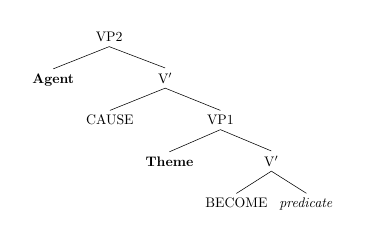
\begin{tikzpicture}[scale=.5]
 \Tree [.VP2 [.\textbf{Agent} ] 
 [.V$'$ [.CAUSE ] 
 [.VP1 [.\textbf{Theme} ] [.V$'$ [.BECOME ] 
 [.\textit{predicate} ] ] ] ] ]
\end{tikzpicture}

\caption{The structure of transitive verbs}
\label{i:tree}
\end{figure} % 匯入結果
\chapter{Discussion}
\label{c:discussion}
\section{Second Level of Title}
This is your discussion. This is your discussion. This is your discussion. This is your discussion. This is your discussion. This is your discussion. This is your discussion. This is your discussion. This is your discussion. This is your discussion. This is your discussion. This is your discussion. This is your discussion. This is your discussion. This is your discussion. 
\subsection{Third Level of Title}
This is your discussion. This is your discussion. This is your discussion. This is your discussion. This is your discussion. This is your discussion. This is your discussion. This is your discussion. This is your discussion. This is your discussion. This is your discussion. This is your discussion. This is your discussion. This is your discussion. This is your discussion. 
\subsubsection{Forth Level of Title}
This is your discussion. This is your discussion. This is your discussion. This is your discussion. This is your discussion. This is your discussion. This is your discussion. This is your discussion. This is your discussion. This is your discussion. This is your discussion. This is your discussion. This is your discussion. This is your discussion. This is your discussion.  % 匯入討論
\chapter{Conclusions}
\label{c:conclusion}

This is your conclusion. This is your conclusion. This is your conclusion. This is your conclusion. This is your conclusion. This is your conclusion. This is your conclusion. This is your conclusion. This is your conclusion. This is your conclusion. This is your conclusion. This is your conclusion. This is your conclusion. This is your conclusion. This is your conclusion. This is your conclusion. This is your conclusion. This is your conclusion. This is your conclusion.  % 匯入結論

% 想要匯入自己加的新章節就打\input{chapters\檔案名},章節會以這邊input的順序呈現,所以請視個人需要調整。

\backmatter

\clearpages
\phantomsection
\addcontentsline{toc}{chapter}{References}


% Your bibliography goes here
\printbibliography[title=References]


\vspace{5.08cm}
\chapter*{\centering Appendix A} % 附錄標題
\addcontentsline{toc}{chapter}{Appendix A} 
% 跟目錄的連結,把最後一個括號裡面的東西改成附錄標題就可以

% 內容從下面開始
Add what you need for appendix here. The way to add a new appendix is to create a new .tex file in the appendix folder and copy what is in this file to that one. After creating the file, we want to include it in the thesis, so you will have to go to line 129 of thesis.tex and follow the instruction. 
% 把附錄引進來,如果還有其他附錄檔案就複製這行程式碼到下一行然後把大括號裡面檔名的部分進行修改即可。
\end{document}
